%%%%%%%%%%%%%%%%%%%%%%%%%%%%%%%%%%%%%%%%%
% University/School Laboratory Report
% LaTeX Template
% Version 3.1 (25/3/14)
%
% This template has been downloaded from:
% http://www.LaTeXTemplates.com
%
% Original author:
% Linux and Unix Users Group at Virginia Tech Wiki 
% (https://vtluug.org/wiki/Example_LaTeX_chem_lab_report)
%
% License:
% CC BY-NC-SA 3.0 (http://creativecommons.org/licenses/by-nc-sa/3.0/)
%
%%%%%%%%%%%%%%%%%%%%%%%%%%%%%%%%%%%%%%%%%

%----------------------------------------------------------------------------------------
%	PACKAGES AND DOCUMENT CONFIGURATIONS
%----------------------------------------------------------------------------------------

\documentclass{article}

\usepackage{polski}
\usepackage[utf8x]{inputenc}
\usepackage{booktabs}
\usepackage{multirow}
\usepackage{caption}

\usepackage[version=3]{mhchem} % Package for chemical equation typesetting
\usepackage{siunitx} % Provides the \SI{}{} and \si{} command for typesetting SI units
\usepackage{graphicx} % Required for the inclusion of images
\usepackage{natbib} % Required to change bibliography style to APA
\usepackage{amsmath} % Required for some math elements 
\usepackage{multirow}

\setlength\parindent{0pt} % Removes all indentation from paragraphs

\renewcommand{\labelenumi}{\alph{enumi}.} % Make numbering in the enumerate environment by letter rather than number (e.g. section 6)

%\usepackage{times} % Uncomment to use the Times New Roman font

%----------------------------------------------------------------------------------------
%	DOCUMENT INFORMATION
%----------------------------------------------------------------------------------------

\title{Ćwiczenie nr 82: Efekt fotoelektryczny} % Title

\author{Rafał \textsc{Grabiański} i Zbigniew \textsc{Królikowski}} % Author name

\date{\today} % Date for the report

\addtolength{\oddsidemargin}{-.875in}
\addtolength{\evensidemargin}{-.875in}
\addtolength{\textwidth}{1.75in}
\addtolength{\topmargin}{-.875in}
\addtolength{\textheight}{1.75in}

\begin{document}

% Please add the following required packages to your document preamble:
% \usepackage{booktabs}
\begin{table}[h]
\begin{tabular}{@{}llllll@{}}
\toprule
\begin{tabular}[c]{@{}l@{}}Wydział:\\ \\ WIEiT\end{tabular}                                    & \multicolumn{2}{l}{\begin{tabular}[c]{@{}l@{}}Imię i nazwisko:\\ Rafał Grabiański\\ Zbigniew Królikowski\end{tabular}}                & \begin{tabular}[c]{@{}l@{}}Rok:\\ \\ II\end{tabular}            & \begin{tabular}[c]{@{}l@{}}Grupa:\\ \\ 7\end{tabular}              & \begin{tabular}[c]{@{}l@{}}Zespół:\\ \\ 7\end{tabular} \\ \midrule
\multicolumn{1}{|c|}{\begin{tabular}[c]{@{}c@{}}PRACOWNIA\\ FIZYCZNA\\ WFiIS AGH\end{tabular}} & \multicolumn{4}{l|}{Temat: Dioda półprzewodnikowa}                                                                                                                                                                                                                                                  & \multicolumn{1}{l|}{Nr ćwiczenia: 123}                     \\ \midrule
\begin{tabular}[c]{@{}l@{}}Data wykonania:\\ \\ \\ 21.10.2014\end{tabular}                     & \begin{tabular}[c]{@{}l@{}}Data oddania:\\ \\ \\ 28.10.2014\end{tabular} & \begin{tabular}[c]{@{}l@{}}Zwrot do poprawy:\\ \\ \\ 18.11.2014\end{tabular} & \begin{tabular}[c]{@{}l@{}}Data oddania: 25.11.2014\\ \\ \\ .\end{tabular} & \begin{tabular}[c]{@{}l@{}}Data zaliczenia:\\ \\ \\ .\end{tabular} & OCENA:                                                  \\ \bottomrule
\end{tabular}
\end{table}

%\maketitle % Insert the title, author and date

% If you wish to include an abstract, uncomment the lines below


%----------------------------------------------------------------------------------------
%	SECTION 1 - CEL ĆWICZENIA
%----------------------------------------------------------------------------------------

\section{Cel ćwiczenia}

Celem naszego ćwiczenia było poznanie własności warstwowych złącz półprzewodnikowych typu p-n. Cel ten miał zostać osiągnięty poprzez wyznaczenie i analizę charakterystyk stałoprądowych dla czterech typów diód: germanowej, krzemowej, świecącej i Zenera.

% If you have more than one objective, uncomment the below:
%\begin{description}
%\item[First Objective] \hfill \\
%Objective 1 text
%\item[Second Objective] \hfill \\
%Objective 2 text
%\end{description}

\subsection{Definicje}
\label{definitions}
\begin{description}
\item[Współczynnik nieidealności]
Wskaźnik mówiący o tym jak bardzo natężenie prądu odbiega od tego wyliczonego na podstawie wzoru dla doskonałej diody Shoeckleya. Współczynnik liczymy na podstawie wzoru: $m = \frac{1}{aU_{T}}$, gdzie $U_{T}$ to stała nazywana napięciem termicznym.
\item[Przerwa energetyczna]
Zakres energii elektronów, dla której w danym materiale są one silnie rozpraszane na atomach i w konsekwencji w układzie nie ma elektronów z energiami w tym zakresie.
\item[Współczynnik stabilizacji]
Stosunek względnej zmiany napięcia do względnej zmiany prądu w diodzie.
\end{description} 

\section{Przebieg pomiarów}
Podczas wykonywania ćwiczenia korzystaliśmy z zestawu składającego się z: czułego przyrządu uniwersalnego V-640, który służył nam jako amperomierz, multimetra służącego jako woltomierz, zestawu czterech diód: germanowej, krzemowej, Zenera i świecącej oraz zasilacza prądu stałego.

Naszym zadaniem było wykonanie pomiarów napięć na poszczególnych diodach przy zadanym napięciu i na bazie tych wyników opracowanie charakterystyki dla wszystkich diód w kierunku przewodzenia oraz zaporowym.
 
\clearpage
%\clearpage

%----------------------------------------------------------------------------------------
%	SECTION 4
%----------------------------------------------------------------------------------------
\section{Wyniki pomiarów}

\begin{table}[htbp]
\begin{center}
\begin{tabular}{|c|c|c|c|c|}
\hline
\multirow{2}{*}{I [A]} & \multicolumn{4}{c|}{Napięcie U[V] diody }\\ \cline{2-5}
 & Ge & Si & Świecąca & Zenera \\ \hline
0.0001 & 0.053 & 0.395 & 2.44 & 0.593 \\ \hline
0.0002 & 0.064 & 0.406 & 2.46 & 0.604 \\ \hline
0.0003 & 0.075 & 0.422 & 2.48 & 0.621 \\ \hline
0.0005 & 0.091 & 0.442 & 2.51 & 0.639 \\ \hline
0.0007 & 0.101 & 0.454 & 2.53 & 0.651 \\ \hline
0.001 & 0.113 & 0.467 & 2.56 & 0.662 \\ \hline
0.002 & 0.136 & 0.491 & 2.62 & 0.682 \\ \hline
0.003 & 0.152 & 0.508 & 2.67 & 0.694 \\ \hline
0.005 & 0.172 & 0.531 & 2.75 & 0.71 \\ \hline
0.007 & 0.186 & 0.546 & 2.8 & 0.72 \\ \hline
0.01 & 0.202 & 0.562 & 2.87 & 0.731 \\ \hline
\end{tabular}
\end{center}
\label{fig:table1}
\caption{Charakterystyka prądowo-napięciowa dla diód połączonych w kierunku przewodzenia}
\end{table}

\begin{table}[h!tbp]
\begin{center}
\begin{tabular}{|c|c|c|c|c|c|c|}
\hline
\multicolumn{2}{|c}{Dioda Ge} & \multicolumn{3}{|c}{Diody inne} & \multicolumn{2}{|c|}{Dioda Zenera} \\ \hline
U[V] & I[$A$] & U[V] & Si I[$A$] & świecąca I[$A$] & I[A] & U[V]\\ \hline
-0.02 & -0.0000095 & -0.1 & -0.000000015 & -0.00000001 & -0.0001 & -10.32 \\ \hline
-0.04 & -0.000015 & -0.2 & -0.000000025 & -0.00000002 & -0.0002 & -10.35 \\ \hline
-0.06 & -0.000015 & -0.3 & -0.000000035 & -0.00000003 & -0.0003 & -10.36 \\ \hline
-0.08 & -0.00002 & -0.5 & -0.00000006 & -0.000000045 & -0.0005 & -10.37 \\ \hline
-0.1 & -0.00002 & -0.7 & -0.00000008 & -0.000000065 & -0.0007 & -10.37 \\ \hline
-0.2 & -0.00002 & -1 & -0.00000011 & -0.000000095 & -0.001 & -10.38 \\ \hline
-0.3 & -0.00002 & -1.5 & -0.00000015 & -0.000000145 & -0.0015 & -10.39 \\ \hline
-0.5 & -0.00002 & -2 & -0.0000002 & -0.0000002 & -0.002 & -10.39 \\ \hline
-0.7 & -0.00002 & -3 & -0.0000003 & -0.0000003 & -0.003 & -10.4 \\ \hline
-1 & -0.00002 & -4 & -0.0000004 & -0.0000004 & -0.004 & -10.41 \\ \hline
-1.5 & -0.00002 & -5 & -0.0000005 & -0.0000005 & -0.005 & -10.42 \\ \hline
-2 & -0.00002 & -6 & -0.0000006 & -0.0000006 & -0.006 & \multirow{5}{*}{brak danych} \\ \cline{1-6}
-3 & -0.00002 & -7 & -0.0000007 & -0.0000007 & -0.007 &\\ \cline{1-6}
-4 & -0.00002 & -8 & -0.0000008 & -0.0000008 & -0.008 &\\ \cline{1-6}
-5 & -0.000025 & -9 & -0.0000009 & -0.0000009 & -0.009 & \\ \cline{1-6}
-6 & -0.000025 & -10 & -0.000001 & -0.000001 & -0.01  &\\ \hline
\end{tabular}
\end{center}
\label{fig:table2}
\caption{Charakterystyka prądowo-napięciowa dla diód połączonych w kierunku zaporowym}
\end{table}

\clearpage

%----------------------------------------------------------------------------------------
%	SECTION 5 - WYNIKI
%----------------------------------------------------------------------------------------

\section{Opracowanie wyników}
\subsection{Charakterystyka prądowo-napięciowa dla polaryzacji przewodzenia}

\begin{figure}[h!]
	\centering
	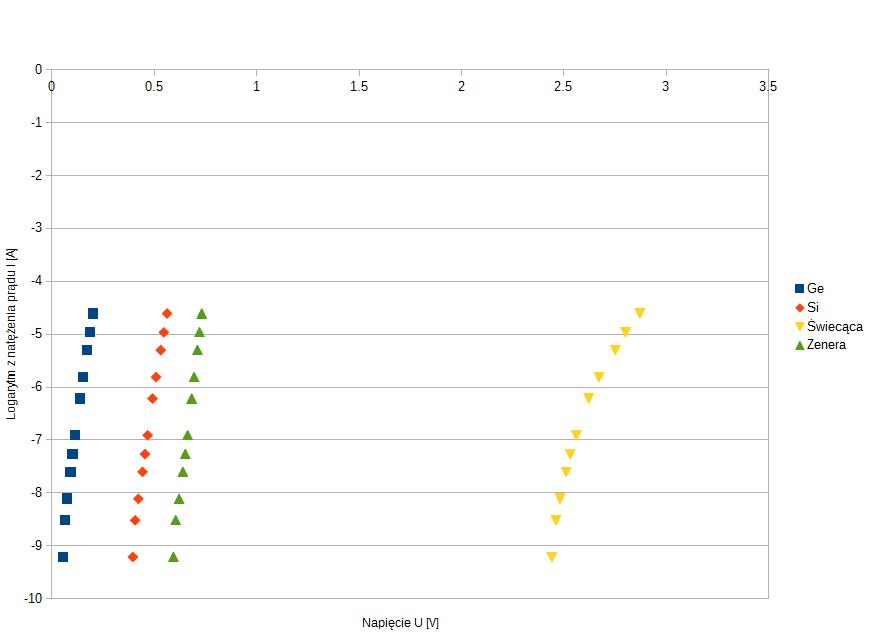
\includegraphics[scale=0.3]{c01new}
	\label{fig:ch01new}
	\caption{Wykres zależności natężenia prądu od napięcia dla diód podłączonych w kierunku przewodzenia $log(I) = f(U)$}
\end{figure}

\subsection{Obliczenie współczynnika idealności dla diody germanowej}

Po wykonaniu zlinearyzowanego wykresu zależności natężenia prądu id napięcia dla diody germanowej, za pomocą arkusza kalkulacyjnego obliczyliśmy, że współczynnik kierunkowy prostej $a = 29.692$. Przyjmując wartość napięcia termicznego $U_{T} = 26mV$, obliczamy wartość współczynnika idealności ze wzoru:
\begin{equation}
	m = \frac{1}{a \cdot U_{T}} 
\end{equation}
Czyli w naszym przypadku: $m = \frac{1}{29.692 \cdot 26*10^{-3}}  = 1.3$.
\begin{figure}[h!]
	\centering
	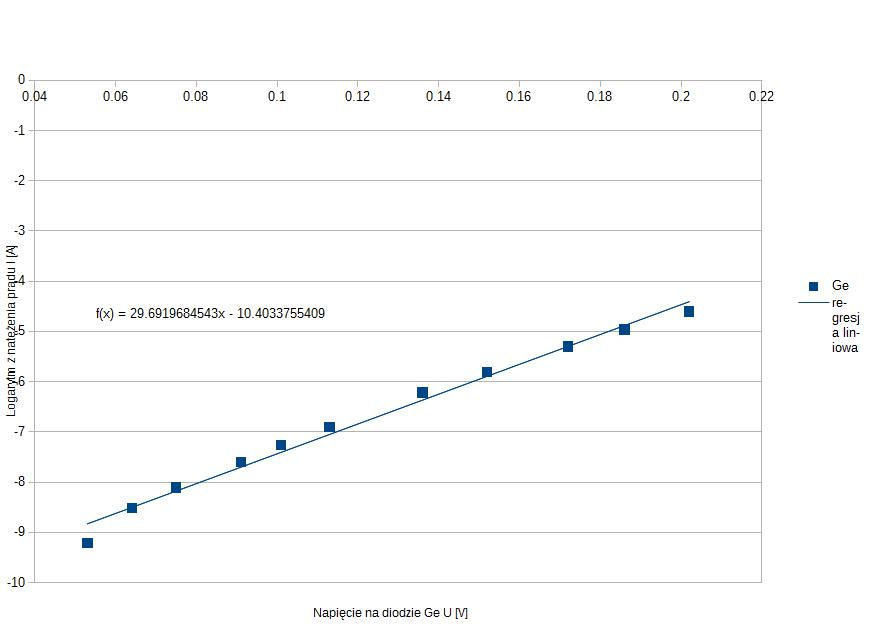
\includegraphics[scale=0.3]{ch02new}
	\label{fig:ch02new}
	\caption{Wykres zależności natężenia prądu od napięcia dla diody Ge}
\end{figure}

\subsection{Analiza przesunięcia charakterystyk diód: krzemowej i germanowej}
Na podstawie wyników z tabeli 1. można obliczyć, że dla danego natężenia różnica w napięciach, które go wywołują jest pomiędzy 0.34V a 0.36V. Natomiast różnica między przerwami energetycznymi dla materiałów, z których wykonane były diody: krzemu (1.11 eV) i germanu (0.67 eV) wynosi 0.44eV.\newline
Można więc wywnioskować, że $\Delta E = e \cdot \Delta U$. Teoretyczna różnica $\Delta E$ powinna wynieść 0.44eV, a wyniosła 0.36eV.

\subsection{Wyznaczenie wartości przerwy energetycznej dla materiału, z którego wykonana jest dioda świecąca}
Przesunięcie charakterystyki diody świecącej względem krzemowej odczytujemy z tabeli: $\Delta U = 2.3 V$.
Wiemy, że $\Delta E = e \cdot \Delta U = 2.1eV$. Wiedząc z kolei, że $E_{Si} = 1.11 eV$ dostajemy $E_{św} = E_{si} + \Delta E = 3.21 eV	$.
Obliczona energia odpowiada energii światła fioletowego (czyli jest w zakresie widzialnym). Podana przerwa energetyczna wskazuje, że dioda została wykonana z azotku galu, który ma przerwę energetyczną wynoszącą 3.4eV.

\subsection{Analiza charakterystyki diody Zenera}
Sprawdziliśmy $\Delta U$ w odniesieniu do diody krzemowej i na podstawie uzyskanych wyników wynosi ono: $0.19V$. Szukamy więc materiału, dla którego $E_{g}$ będzie równe 1.3eV. W przybliżeniu tyle wynosi przerwa energetyczna dla arsenku galu (1.43eV).

\subsection{Charakterystyki I = f(U) dla diod połączonych w kierunku zaporowym}

\begin{figure}[h]
	\centering
	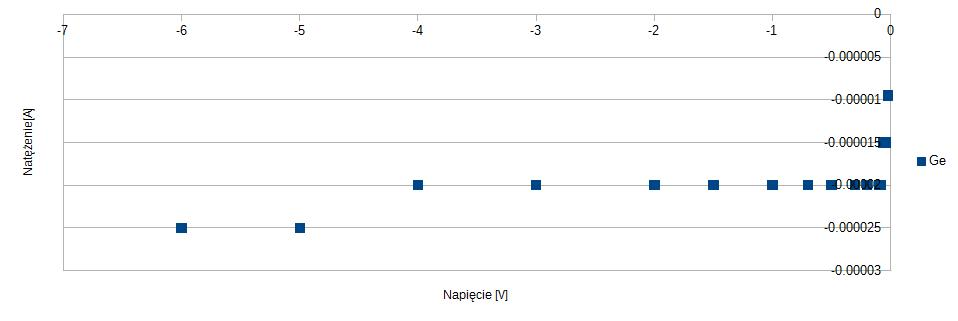
\includegraphics[scale=0.3]{lab02ch03}
	\label{fig:ch03}
	\caption{Zależność  natężenia prądu od napięcia w kierunku zaporowym dla diody Ge}
\end{figure}

\begin{figure}[h]
	\centering
	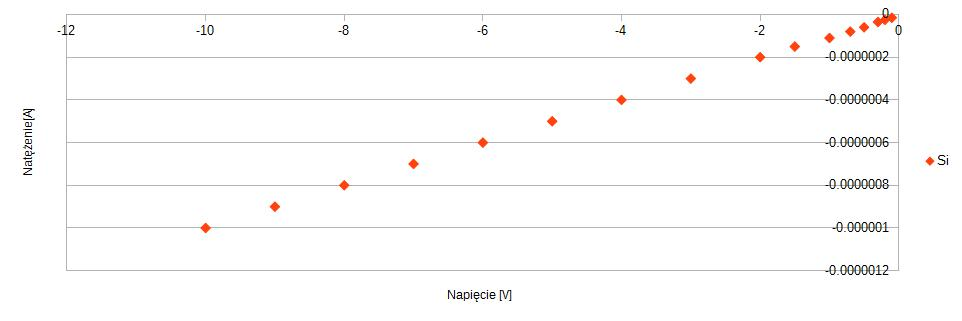
\includegraphics[scale=0.3]{lab02ch04}
	\label{fig:ch03}
	\caption{Zależność  natężenia prądu od napięcia w kierunku zaporowym dla diody Si}
\end{figure}

\begin{figure}[h]
	\centering
	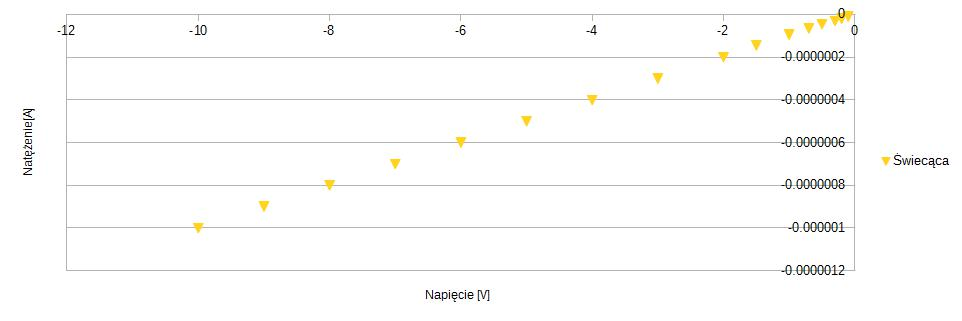
\includegraphics[scale=0.3]{lab02ch05}
	\label{fig:ch03}
	\caption{Zależność  natężenia prądu od napięcie w kierunku zaporowym dla diody LED}
\end{figure}

\begin{figure}[h]
	\centering
	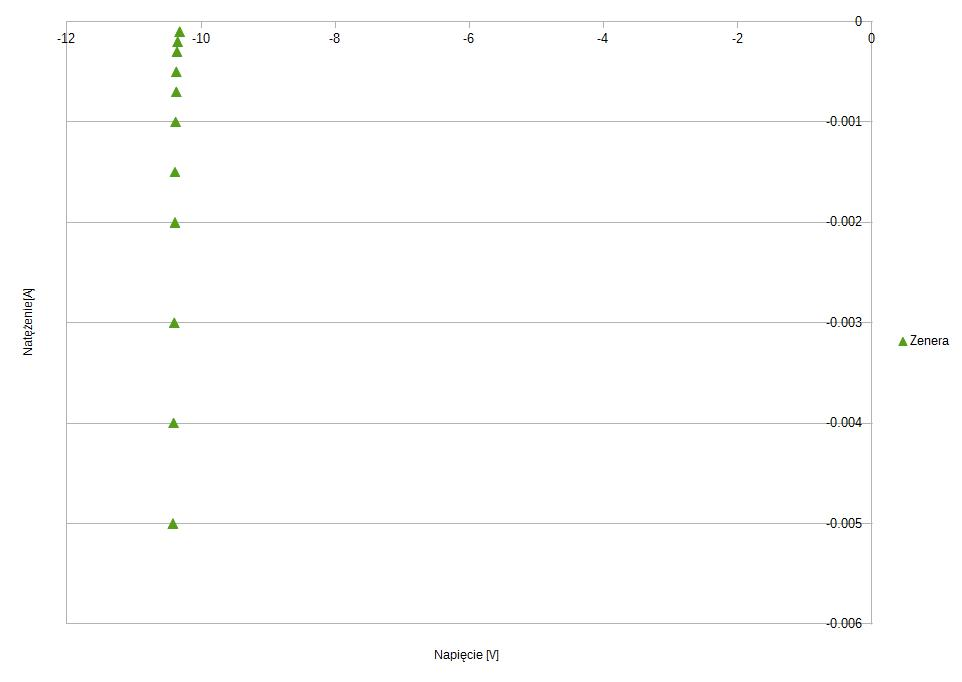
\includegraphics[scale=0.3]{lab02ch06}
	\label{fig:ch03}
	\caption{Zależność  natężenia prądu od napięcie w kierunku zaporowym dla diody Zenera}
\end{figure}

\subsection{Określenie napięcia stabilizowanego $U_{Z}$ dla diody Zenera}

Tak jak według instrukcji, jako napięcie stabilizowane określamy takie napięcie, dla którego prąd płynący w kierunku zaporowym dla diody wyniósł $5mA$. Odczytując dane z tabeli: $U_{z} = 10.42 V$

\subsection{Obliczenie współczynnika stabilizacji diody Zenera}

Współczynnik stabilizacji to iloraz oporności dynamicznej do oporności statycznej, dla kierunku zaporowego.

\begin{equation}
	R = \frac{U_{z}}{I_{0}}
\end{equation}
\begin{equation}
	r = \frac{\Delta U}{\Delta I}
\end{equation}
\begin{equation}
	Z = \frac{r}{R}
\end{equation}

\[R = \frac{10.42V}{0.005A} = 2084 \frac{V}{A} \]
\[r = \frac{0.1 V}{0.0049 A} = 20.41 \frac{V}{A}\]
\[Z = \frac{r}{R} = \frac{20.41}{2084} \approx 0.010\]

%----------------------------------------------------------------------------------------
%	SECTION 6
%----------------------------------------------------------------------------------------
\section{Wnioski}

Wyniki doświadczenia, także w postaci wykresu charakterystyk potwierdziły poprawność modelu złącza pn a także właściwości poszczególnych rodzajów diód. Udało się zaobserwować tzw. "napięcie progowe" czyli napięcie od którego można nałożyć na funkcję asypmotykę liniową, oraz przebicie lawinowe dla diody Zenera, umożliwiające jej pracę w charakterze stablizacyjnym (np. w prostowniku, równolegle do kondensatora za mostkiem Graetza). Pozostałe diody nie uległy temu zjawisku pomimo napięcia dochodzącego do 10V co świadczy o ich specyficznej konstrukcji, adekwatnej do zastosowania. Warto zauważyć, że w układzie pozornie została zastowana dioda niebieska, za której odkrycie w tym roku przyznano Nagrodę Nobla w dziedzinie Fizyki dla Isamu Akasaki, Hiroshi Amano, Shūji Nakamura, wyniki doświadczenia scharakteryzowały ten materiał jako azotek galu(o przerwie energetycznej 3.4 eV), co zgadza się z teorią. Dla diody Zenera otrzymany materiał to arsenek galu.


%----------------------------------------------------------------------------------------
%	BIBLIOGRAPHY
%----------------------------------------------------------------------------------------

\bibliographystyle{apalike}

\bibliography{sample}
%----------------------------------------------------------------------------------------


\end{document}
